\documentclass{beamer}
%Information to be included in the title page:
\title{Gradient Descent}
\author{Enbao Cao \& Ayaan Dhuka}
\institute{Multivariable Calculus}
\date{4/26/2024}

\usepackage{amsmath}
\usepackage{amssymb}
\usepackage{commath}

\usetheme{Darmstadt}

\iffalse
\makeatother
\setbeamertemplate{footline}
{
  \leavevmode%
  \hbox{%
  \begin{beamercolorbox}[wd=.4\paperwidth,ht=2.25ex,dp=1ex,center]{author in head/foot}%
    \usebeamerfont{author in head/foot}\insertshortauthor
  \end{beamercolorbox}%
  \begin{beamercolorbox}[wd=.6\paperwidth,ht=2.25ex,dp=1ex,center]{title in head/foot}%
    \usebeamerfont{title in head/foot}\insertshorttitle\hspace*{3em}
    \insertframenumber{} / \inserttotalframenumber\hspace*{1ex}
  \end{beamercolorbox}}%
  \vskip0pt%
}
\makeatletter
\setbeamertemplate{navigation symbols}{}
\fi

\begin{document}

\frame{\titlepage}

\begin{frame}
\frametitle{Gradient Descent}

goal: find $\underset{x, y}{\min}$ $f(x,y)$ and the corresponding optimal $\textbf{r}^*=<x,y>$. 

\vspace{0.2cm}
moving in the direction of steepest descent, which is the negative of the gradient.

\vspace{0.2cm}

    \begin{center}
    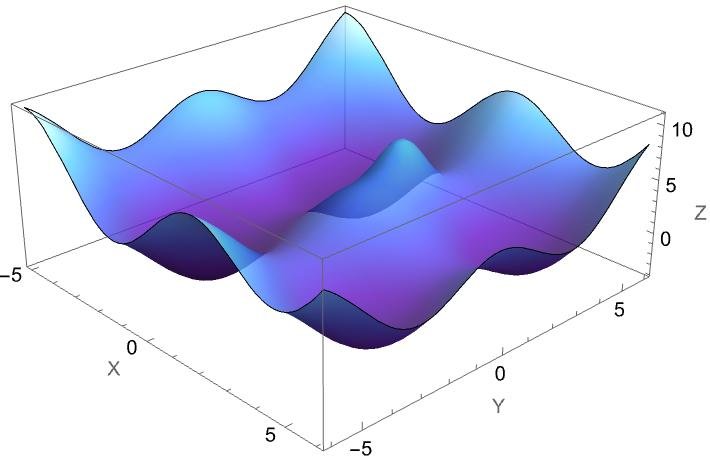
\includegraphics[width=6cm]{example}
    \end{center}
\end{frame}

\begin{frame}
\frametitle{Formulation}

% this is the slide for a general explanation

iterative step:

$$\textbf{r}_{n+1}=\textbf{r}_{n}-\gamma \hspace{0.1cm} \frac{\nabla F(\textbf {r}_n)}{\norm{\nabla F(\textbf{r}_n)}}$$

% mention Goldilocks zone for learning rate (Slide 7)
\begin{align*}
    \textbf{r}_n& \textnormal{: point on the }n^{th}  \textnormal{ iteration, expressed as a vector.}\\
    \gamma& \textnormal{: learning rate. analogous to "step size" for Euler method.}\\
    \nabla F& \textnormal{: gradient of function F}
\end{align*}

\end{frame}


\begin{frame}
\frametitle{Features}

\begin{itemize}
    \item computationally cheap iterations
    \item fast for convex problems (convex: only one minimum, so global guaranteed)
\end{itemize}

\end{frame}


\begin{frame}
\frametitle{Problems}

\begin{itemize}
    \item cannot handle non-differentiable functions
    % absolute value is used in L1 regularization, a process that takes place in a specific regression
    \item cannot guarantee a global minimum
    % random sampling used in advanced optimization algorithms
    % stochastic gradient descent (SGD), mini-batch gradient descent, and momentum-based methods
\end{itemize}

\end{frame}

\begin{frame}
\frametitle{Easy Application: Paraboloid}

% Python implementation of gradient descent on the paraboloid $z=x^2+y^2$ (convex surface).
% gradient descent is easily performed

$$f(x,y)=x^2+y^2$$

\begin{figure}
    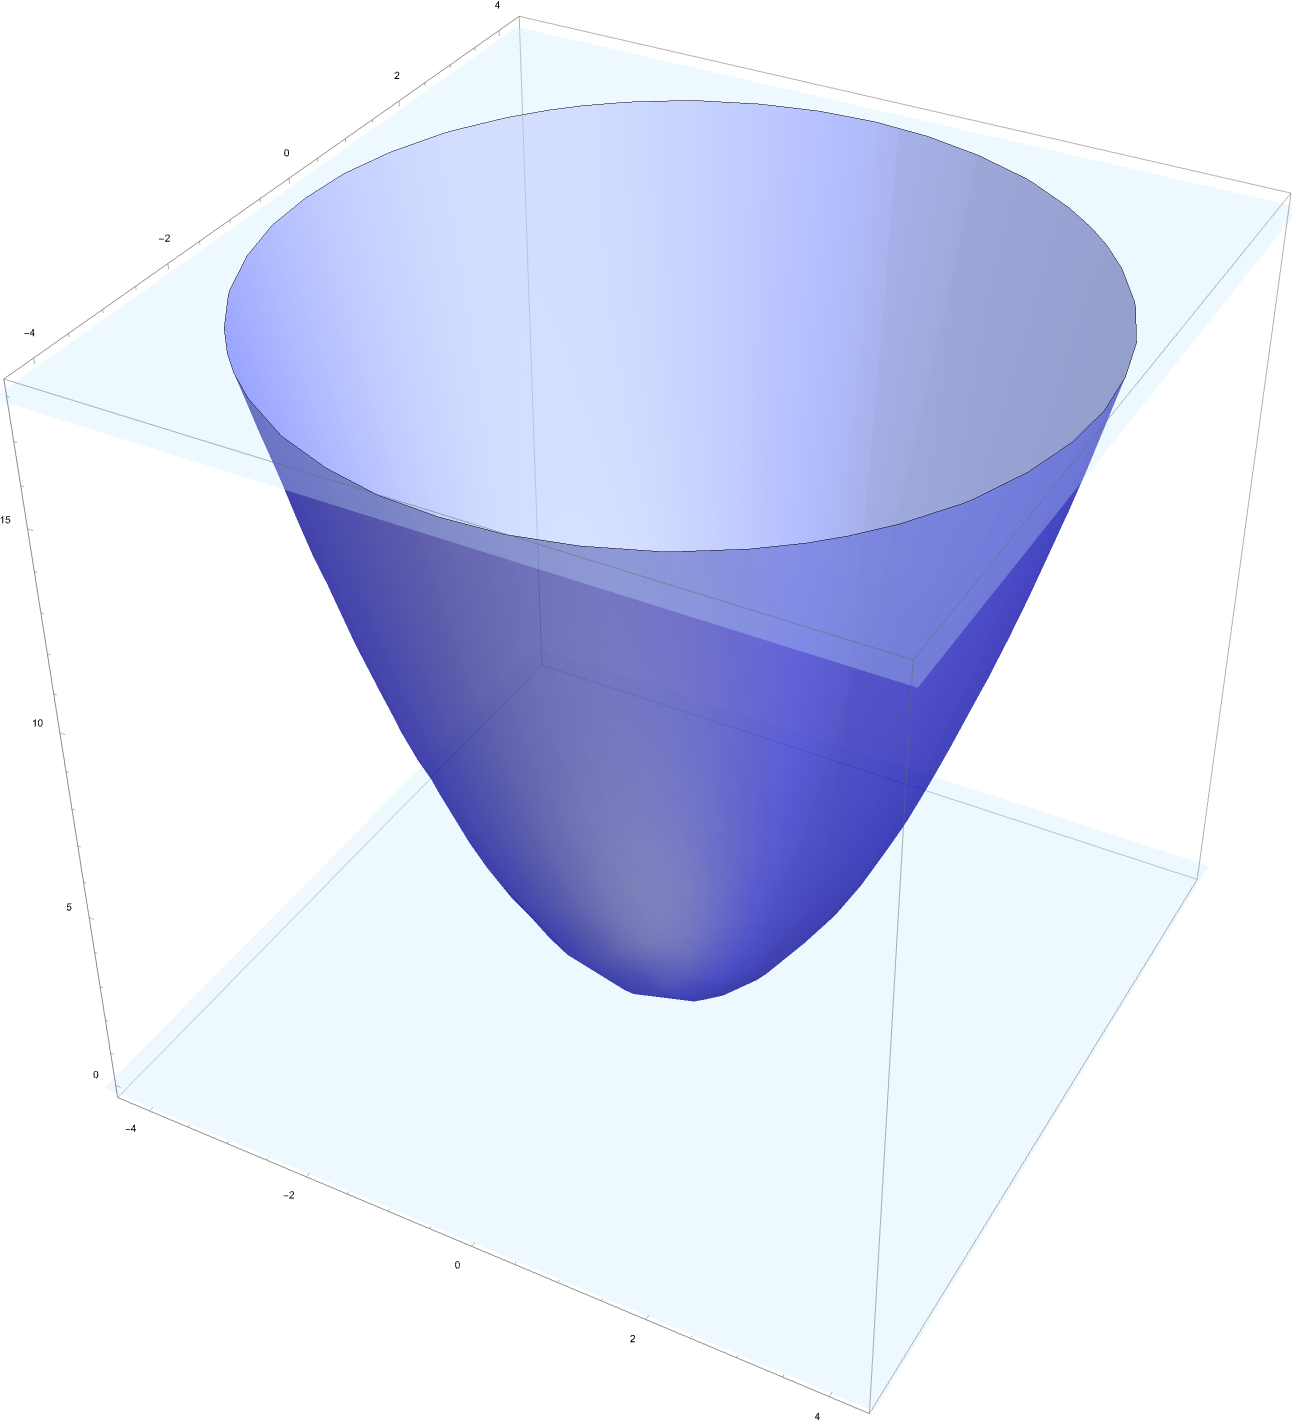
\includegraphics[height=5cm]{paraboloid}
    \hspace{0.8cm}
    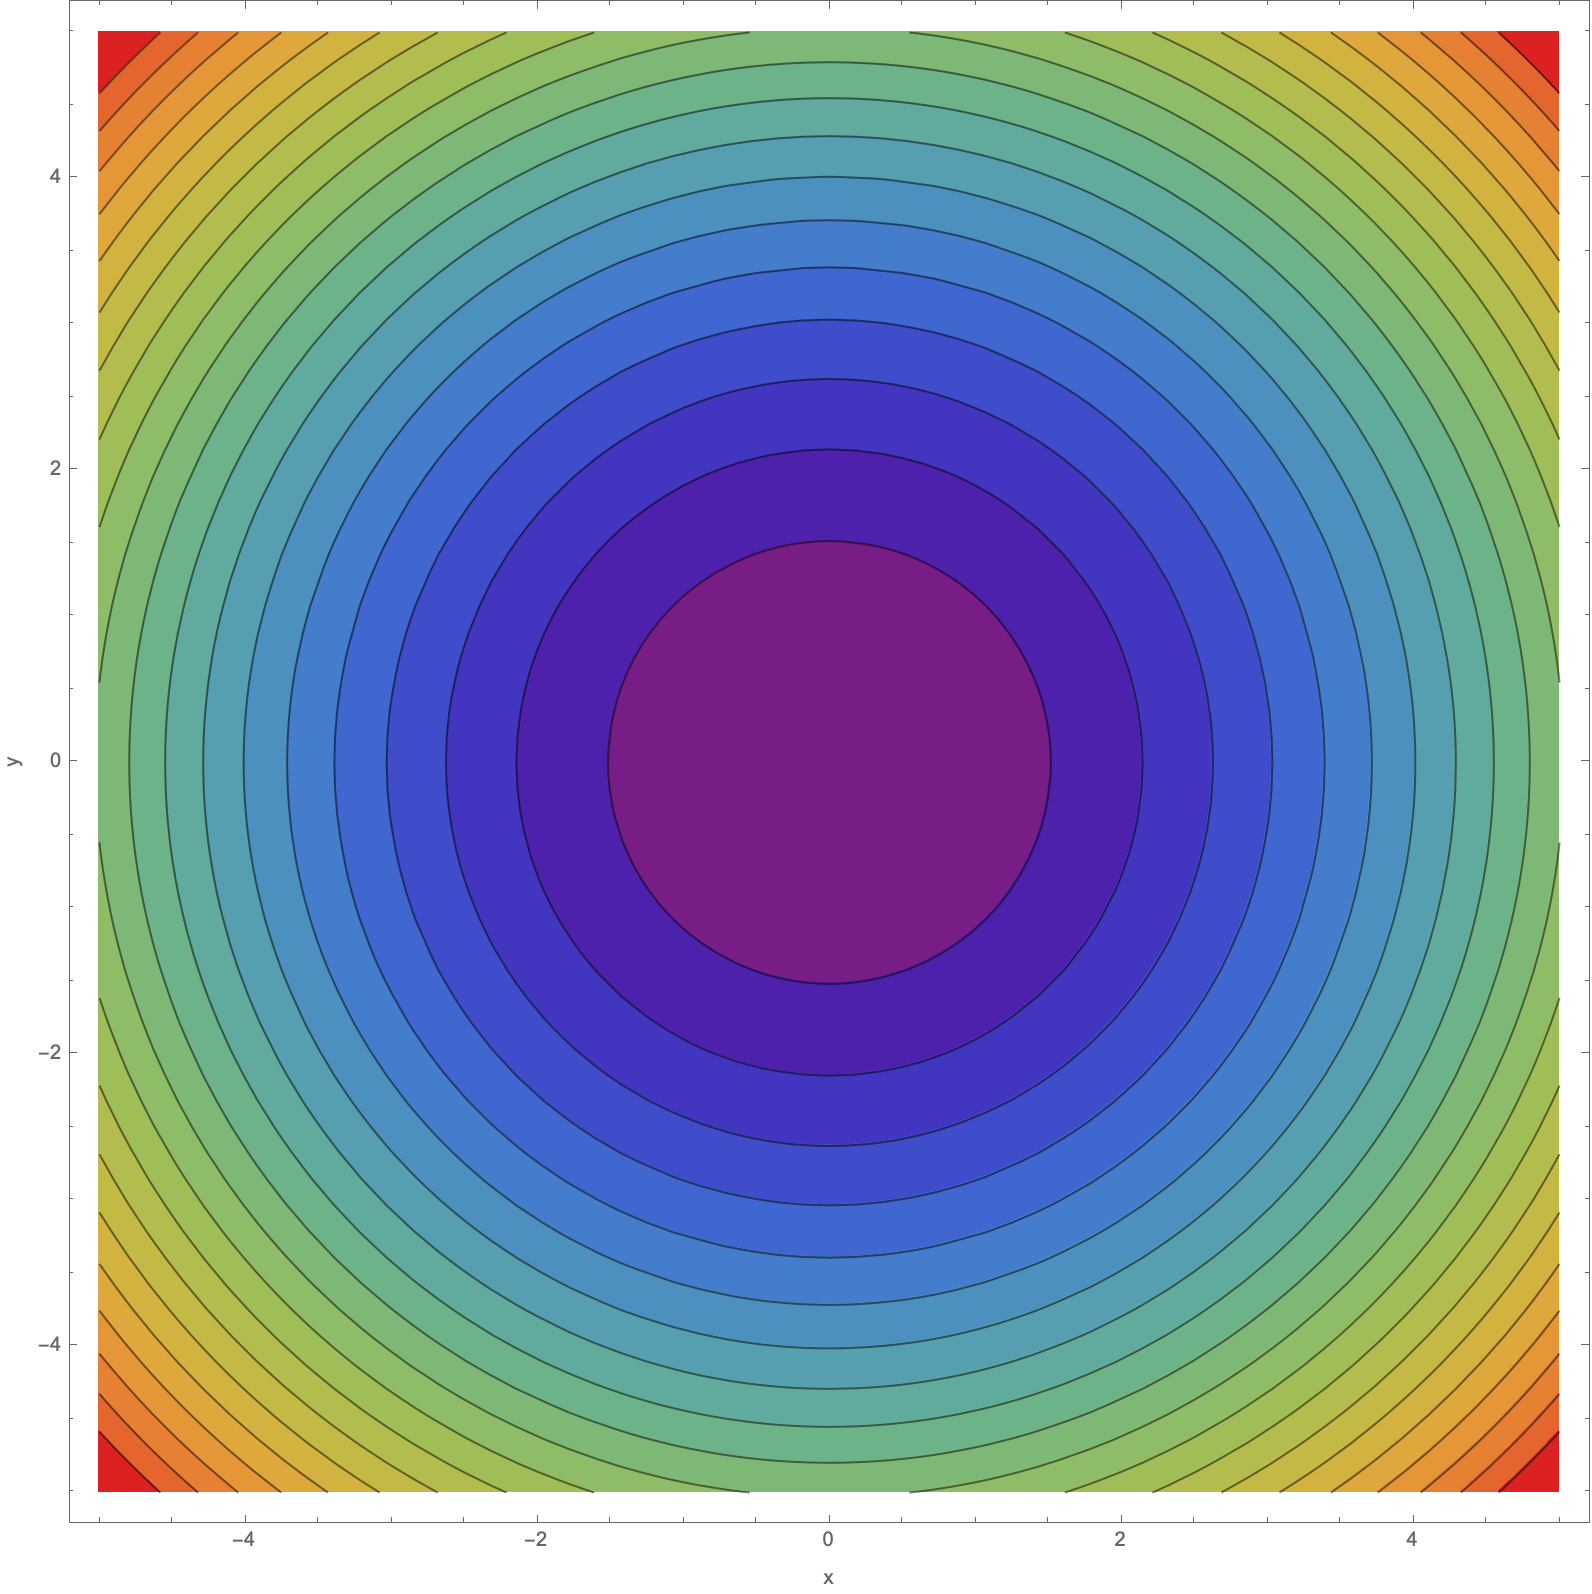
\includegraphics[height=5cm]{paraboloid_levelset}
\end{figure}

\end{frame}

\begin{frame}
\frametitle{Easy Application: Learning Rates}

$100$ iterations of gradient descent were simulated.

$\gamma=5,25,100$ respectively for the figures below.

\begin{figure}
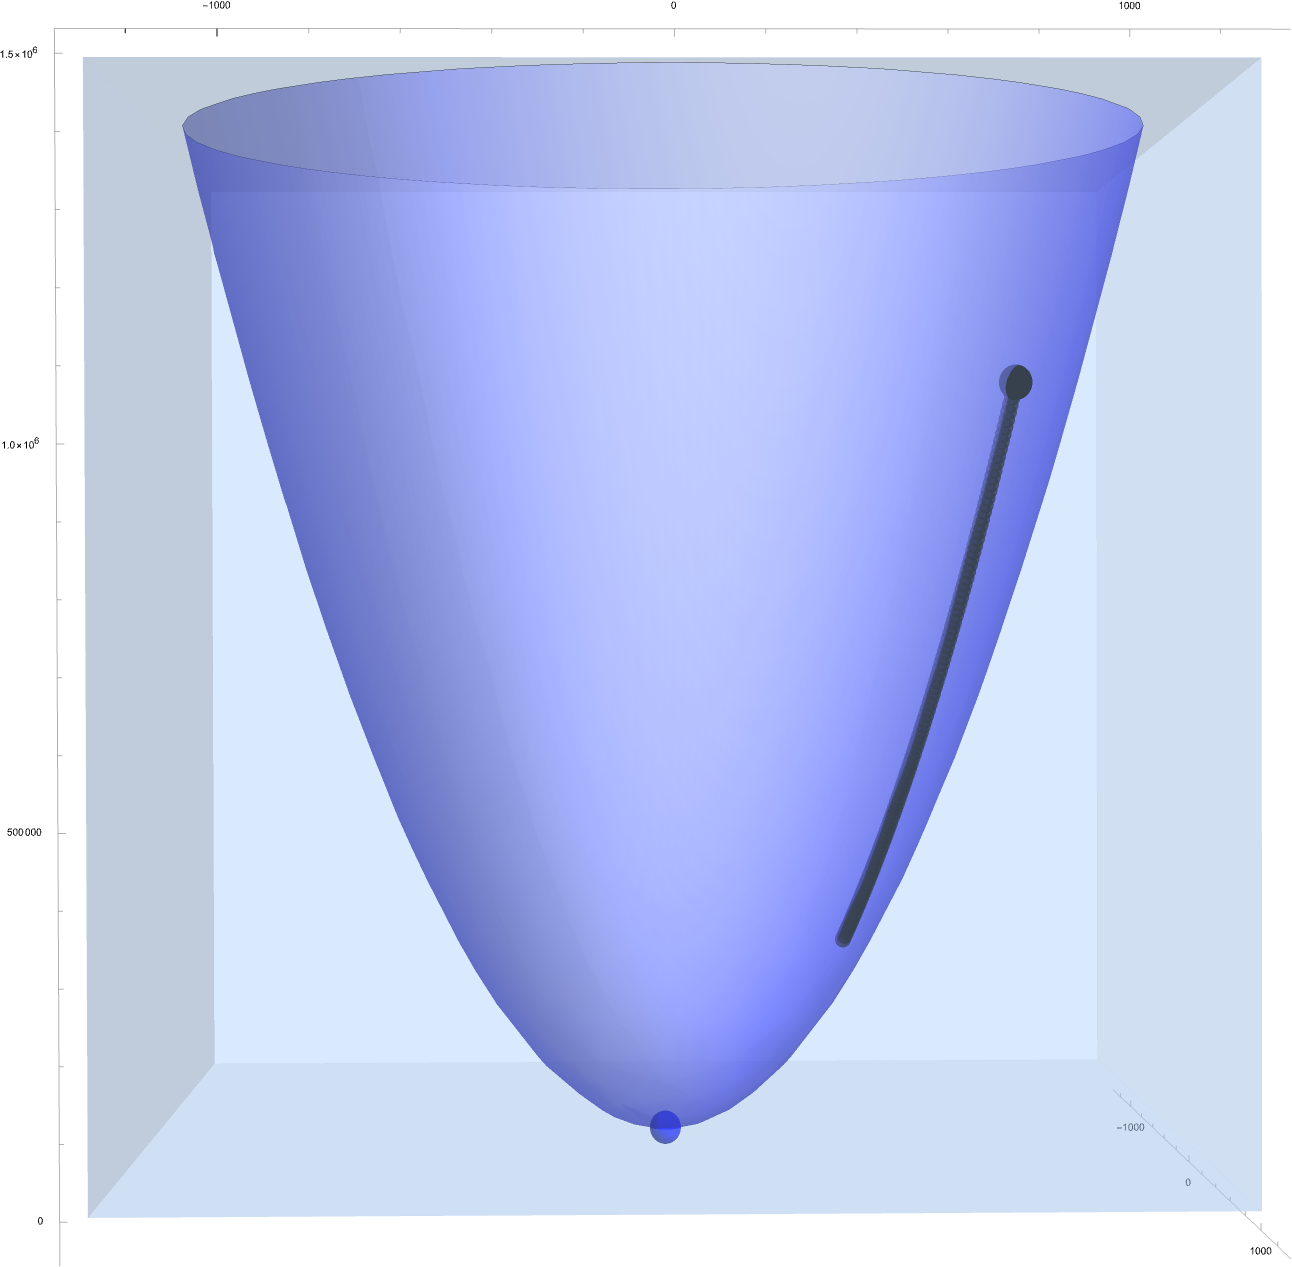
\includegraphics[height=3.3cm]{learning_rate1}
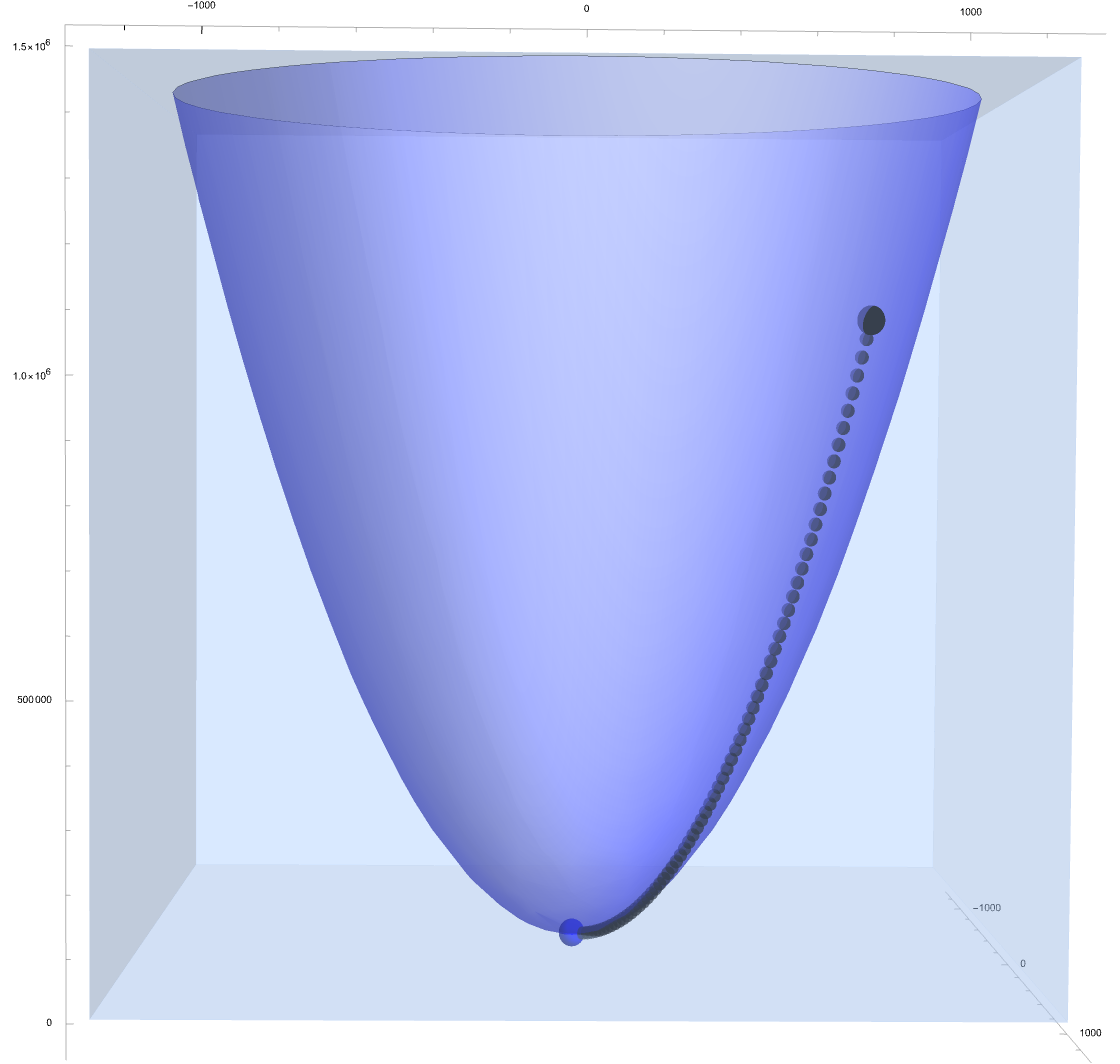
\includegraphics[height=3.3cm]{learning_rate2}
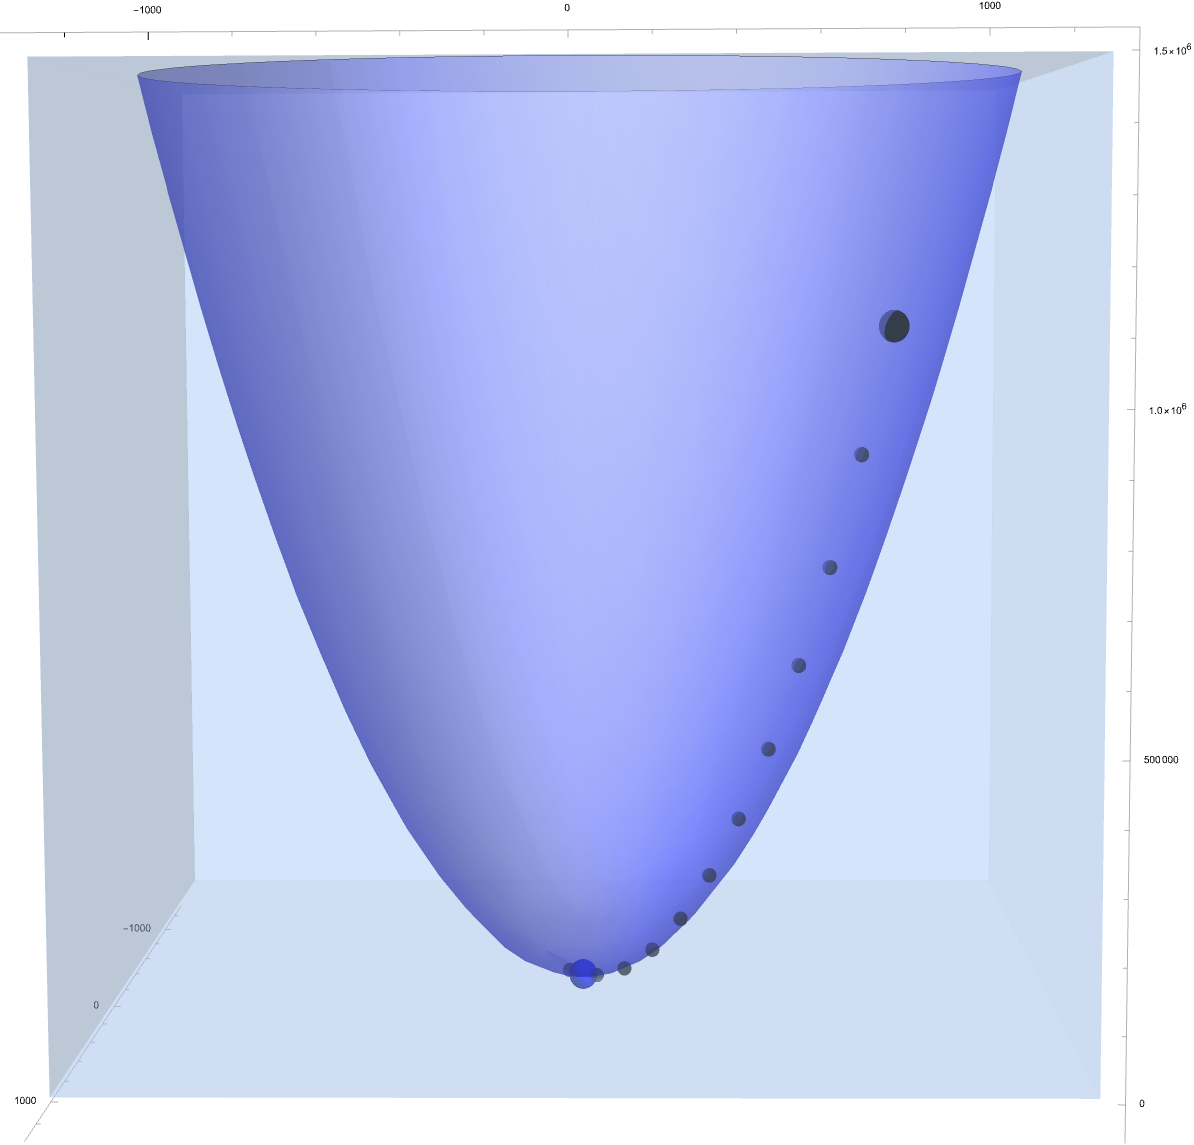
\includegraphics[height=3.3cm]{learning_rate3}
\end{figure}

\end{frame}

\begin{frame}
\frametitle{Non-Trivial Application: More Realistic Surface}

% describe the surface here. describe where the big dip is supposed to be and how we made it that way. problem: many different mins. iterative starting from one starting point can lead to local min, but not extreme min.

$$f(x,y)=2\sin(x)+\cos(y)-8e^{-(x-2)^2-(y-1)^2}+0.1(x^2+y^2)$$

% trigonometric functions, exponential function, quadratic terms

\begin{figure}
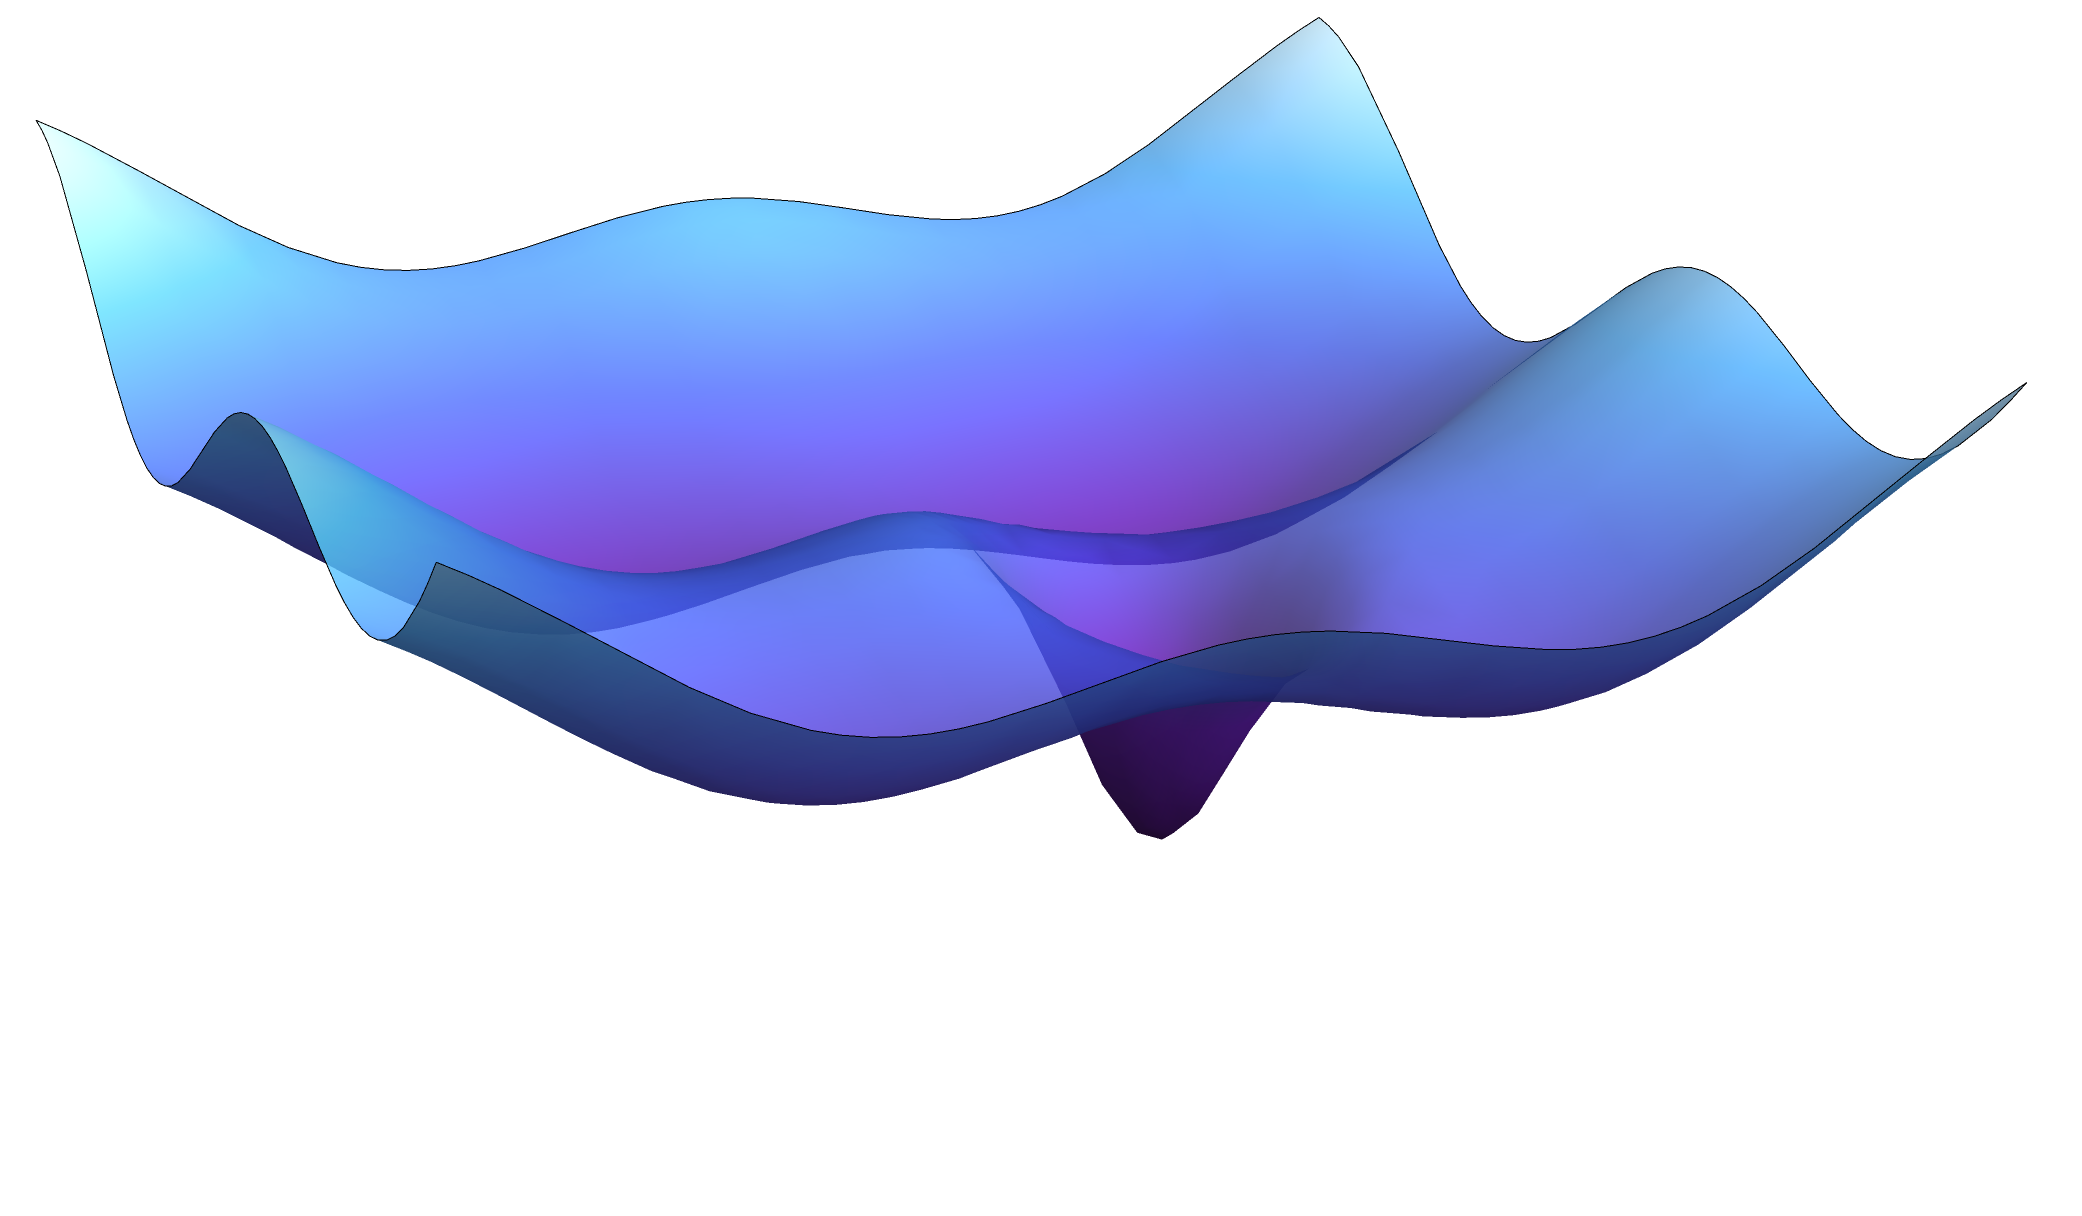
\includegraphics[height=3.7cm]{landscape}
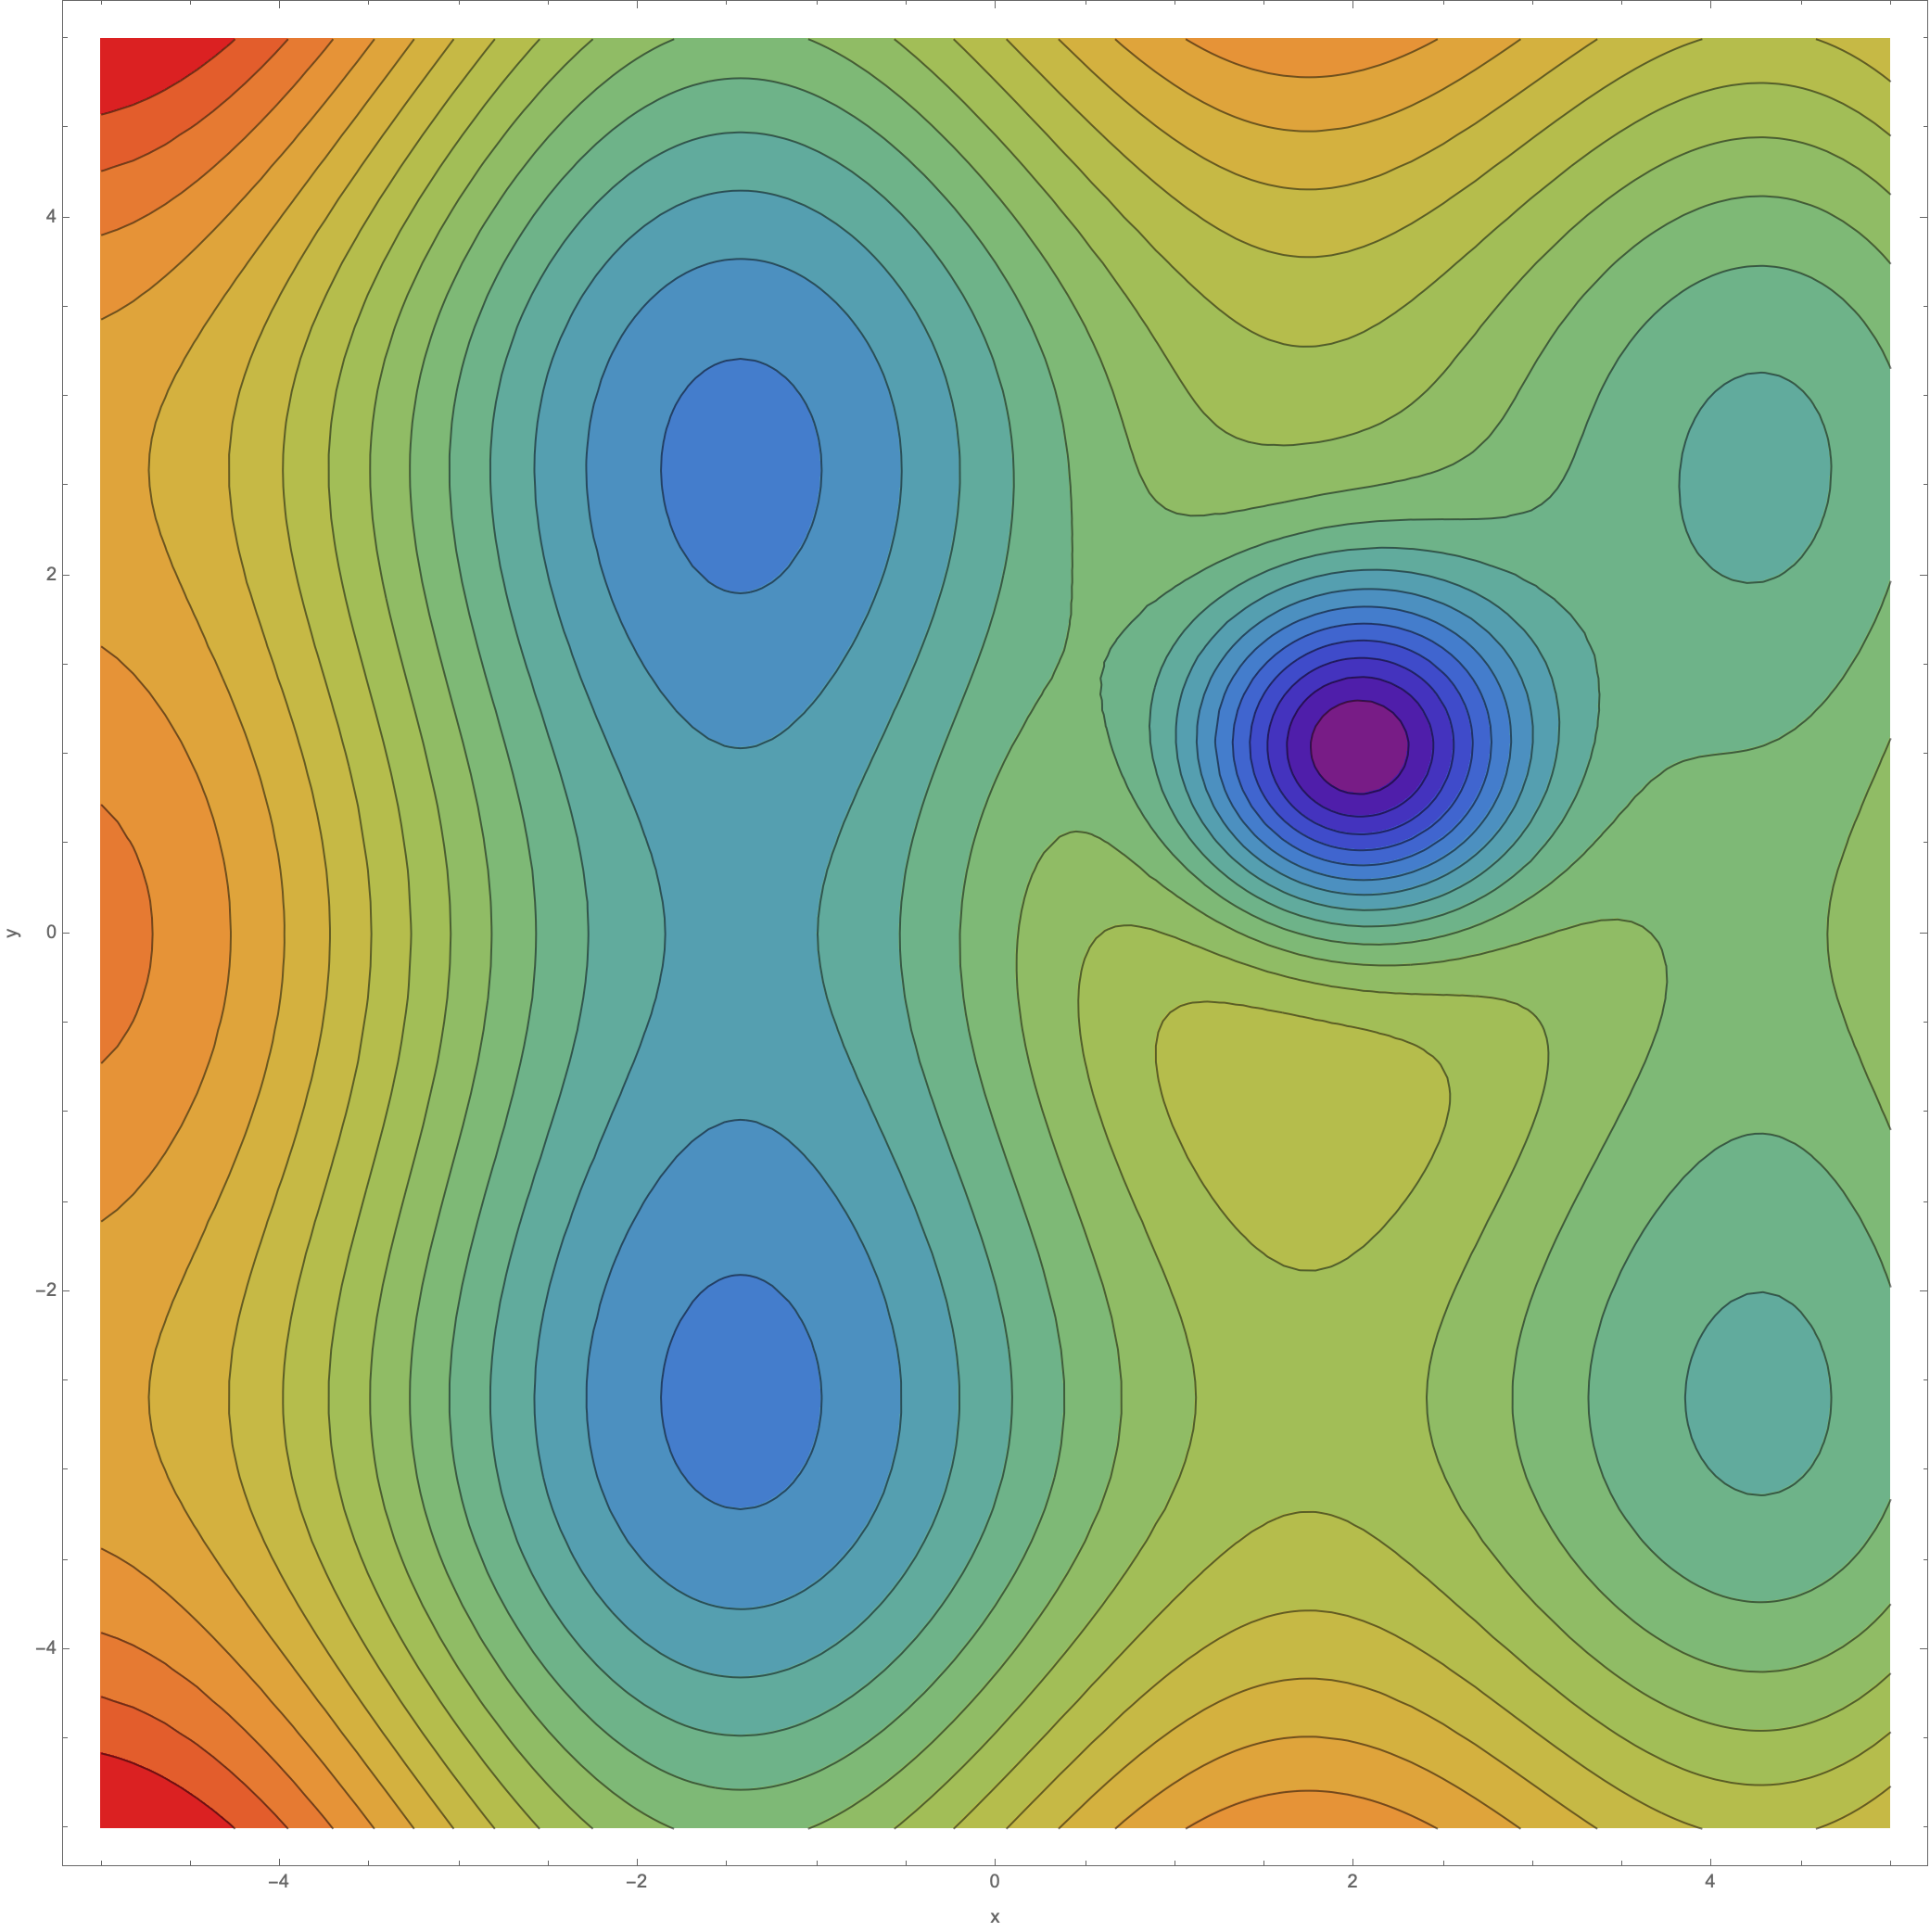
\includegraphics[height=3.7cm]{landscape_levelset}
\end{figure}


\end{frame}

\begin{frame}
\frametitle{Non-Trivial Application: Random Sampling}

% mathematica FindMinimum function, starting point (0, 0)
% vs our function, 100 different starting points
   
% how many iterations

\begin{figure}
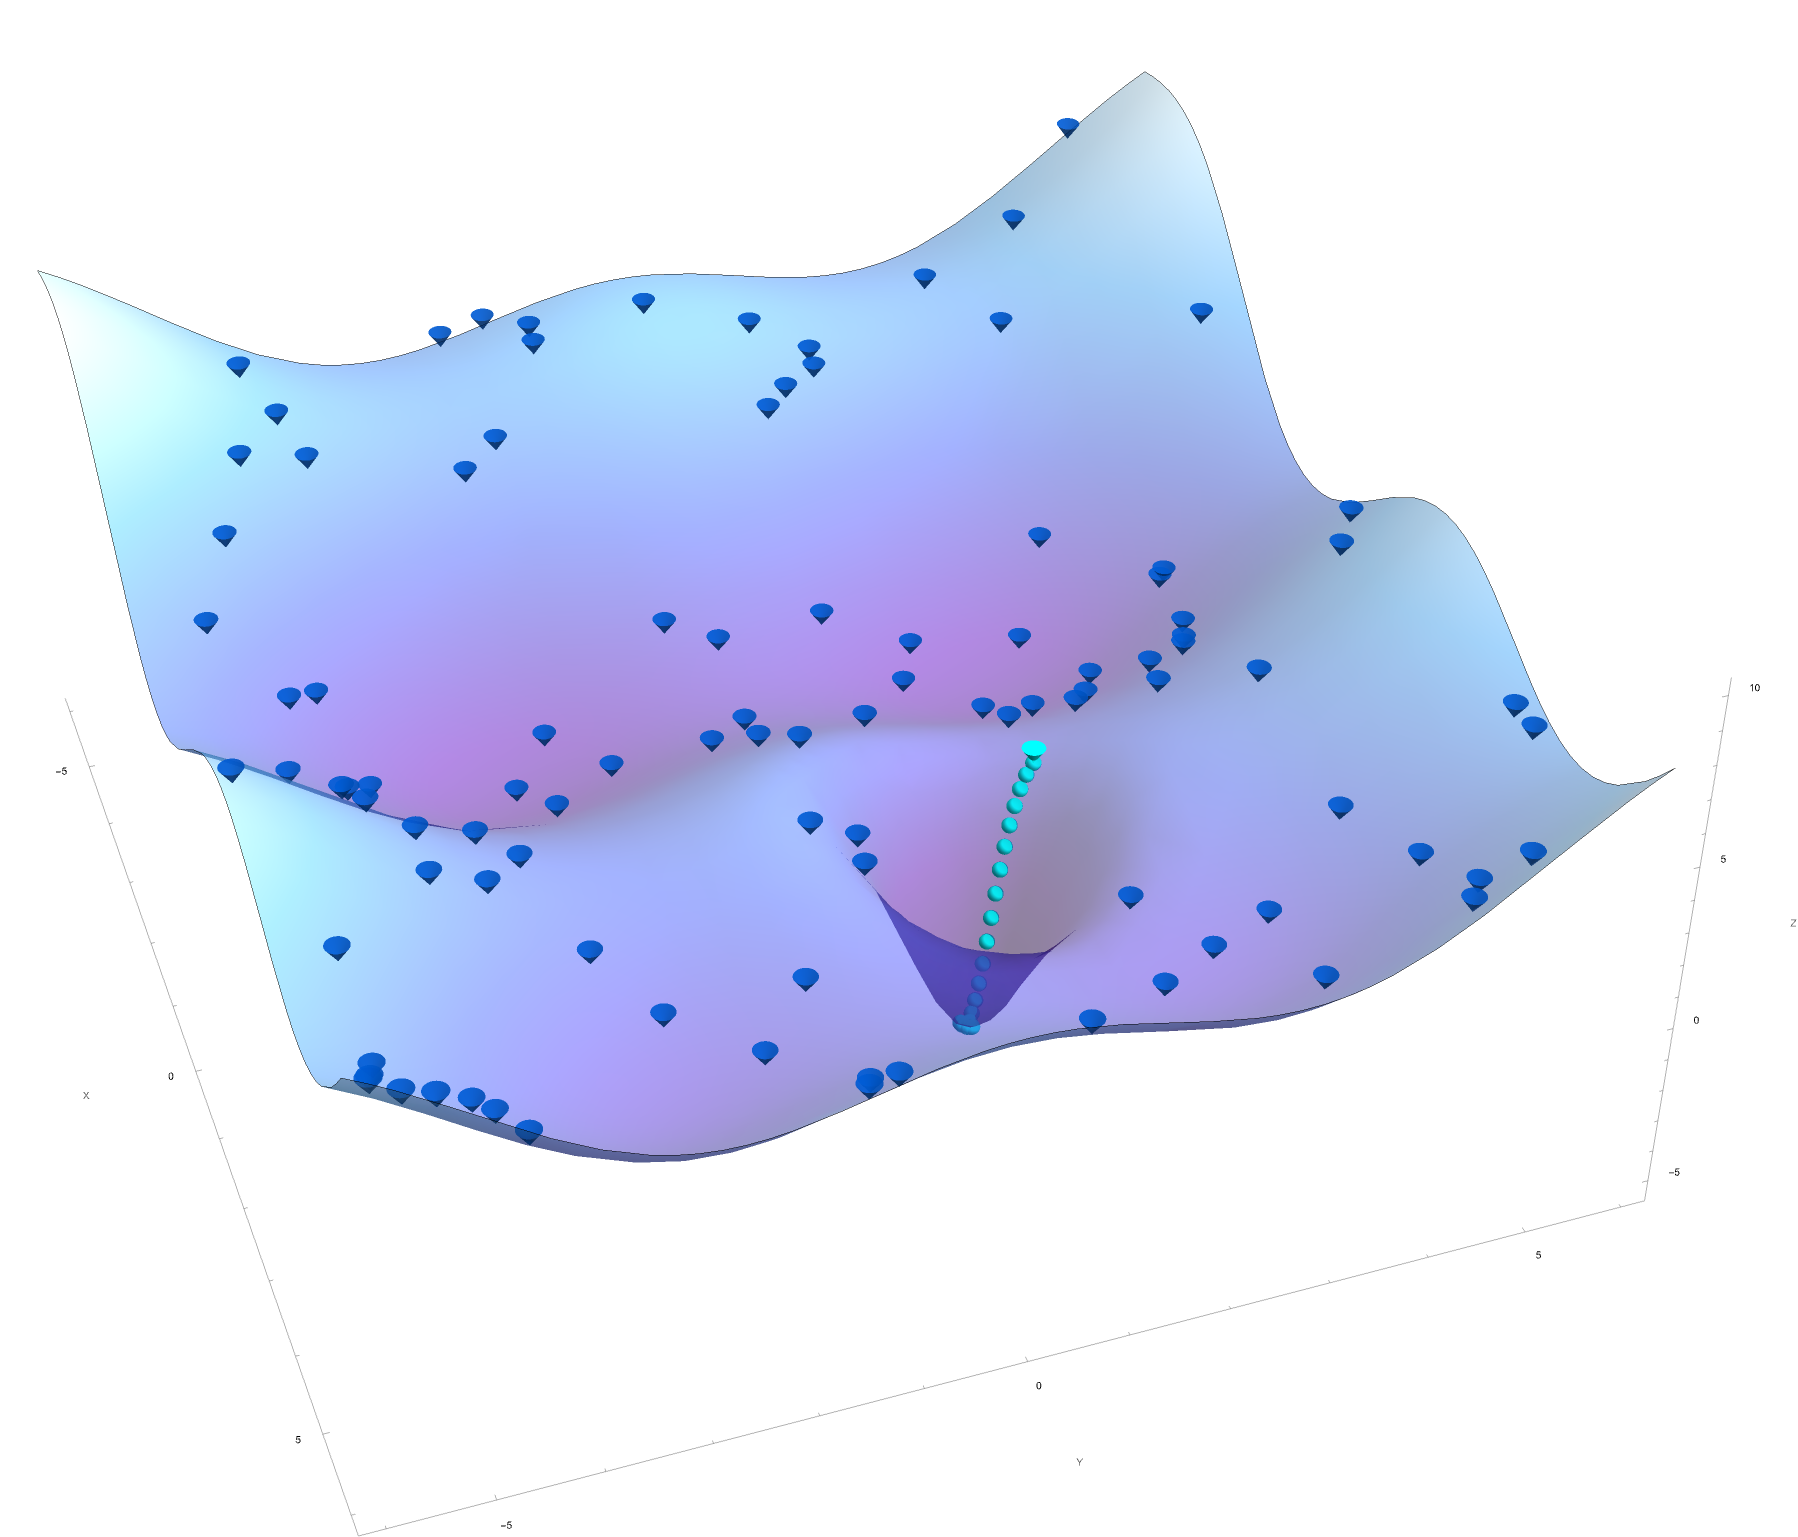
\includegraphics[height=4.2cm]{samples}
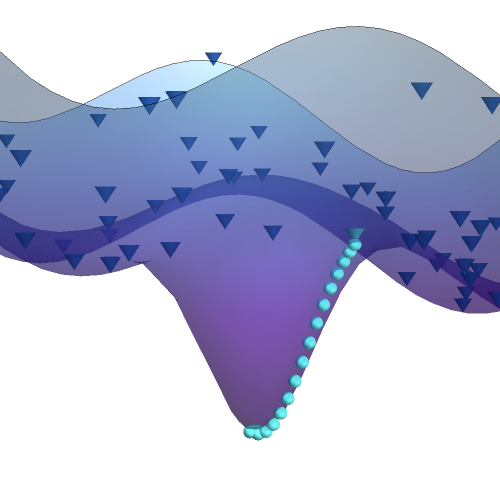
\includegraphics[height=4.2cm]{samples_detail}
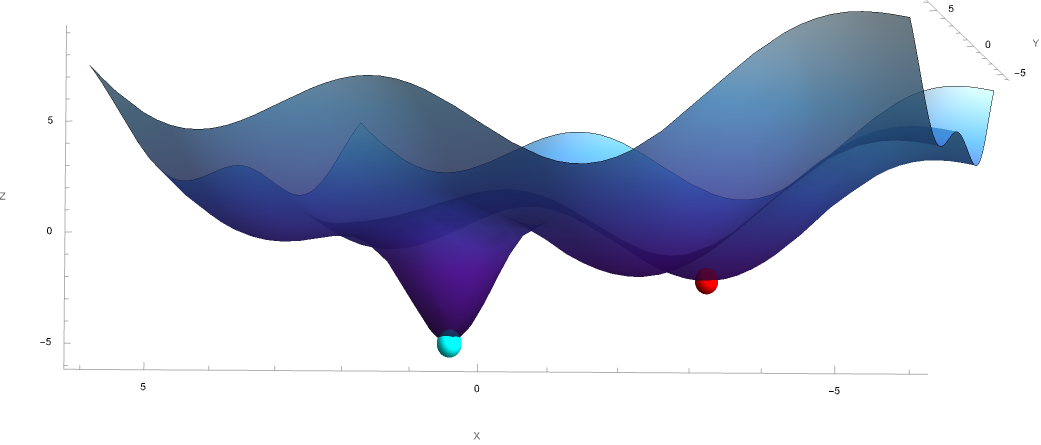
\includegraphics[height=2.4cm]{two_mins}
\end{figure}

\end{frame}

\begin{frame}
\frametitle{Extensions}

Interactive Demo (Cut to Ayaan's App)

\end{frame}

\begin{frame}
\frametitle{Wrap-up}

% n-dimensional
% 3-d, n-dimensional, machine learning millions or billions of parameters
% para (I forgot what this means)

%optimizing parameters, large datasets
% therefore, a problem right now is making it efficient
% gpt3 to gpt4 to gpt5 is just increasing the data required.
% stochastic gradient descent, mini-batch gradient descent), tuning hyperparameters, or applying regularization techniques to prevent overfitting.

\begin{itemize}
    \item lots of parameters for real-world uses
    \item picking the right algorithm and tools
\end{itemize}

\end{frame}

\begin{frame}
\frametitle{Credit}

Visual aids were generated in Mathematica.
\vspace{0.5cm}

Algorithms and demo were implemented in Python. 
\vspace{0.5cm}

The notebook and source code can be found on the repository.
\vspace{0.5cm}

Enbao: Presentation Visualization, Presentation Format
\\
Ayaan: Application 1 Code, Application 2 Code, Simulation Code
\\
Together: Presentation Content

\vspace{0.5cm}

\end{frame}

\end{document}